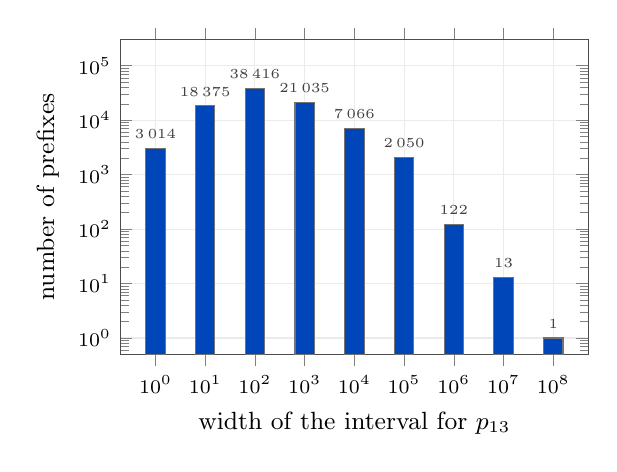
\begin{tikzpicture}
\begin{axis}[width=0.62\textwidth, height=0.46\textwidth, ybar, bar width=7pt, ymode=log, log origin=infty,
  ymin=0.5, ymax=3e5, xmin=-0.7, xmax=8.7,
  xtick={0,...,8}, xticklabels={$10^0$,$10^1$,$10^2$,$10^3$,$10^4$,$10^5$,$10^6$,$10^7$,$10^8$},
  x tick label style={font=\scriptsize}, y tick label style={font=\scriptsize},
  ylabel={\small number of prefixes}, xlabel={\small width of the interval for $p_{13}$},
  grid=major, grid style={black!8}, axis line style={black!70},
  nodes near coords={\pgfmathprintnumber[fixed, precision=0, 1000 sep={\,}]{\pgfplotspointmeta}},
  nodes near coords style={font=\tiny, text=black!75, anchor=south}, point meta=rawy]
\addplot[fill=blue!45!teal, draw=black!55] coordinates {(0,3014) (1,18375) (2,38416) (3,21035) (4,7066) (5,2050) (6,122) (7,13) (8,1)};
\end{axis}
\end{tikzpicture}
